
\chapter{Project Management}

\section{Risk Assessment}

\begin{longtable}[ht]{ p{.2\textwidth} p{0.06\textwidth}  p{0.06\textwidth} p{0.06\textwidth} p{0.5\textwidth}}
  \toprule
  \textbf{Risk}
   & \textbf{Loss}
   & \textbf{Prob}
   & \textbf{Risk}
   & \textbf{Mitigation}
  %
  \\\midrule\midrule
  Laptop damaged or lost
   & 3
   & 1
   & \cellcolor{orange!50} 5
   & All work is stored using version control and periodic backups will be
  made and stored locally and in cloud storage. I have other devices that
  could be used to continue development.
  %
  \x
  Difficulty with blockchain development
   & 2
   & 3
   & \cellcolor{orange!50} 6
   & I will seek advice from my supervisor about how to tackle certain problems
  and if necessary, what aspects of my project I should change.
  %
  \x
  The application is not finished
   & 1
   & 3
   & \cellcolor{green!30} 3
   & Using agile development will ensure that I will at least have a minimal
  working application. If I feel that I am running out of time, I will focus
  on expanding test cases and improving the write-up.
  %
  \x
  No suitable large scale test environment
   & 2
   & 5
   & \cellcolor{red!40} 10
   & I do not have the infrastructure to test this project on a large network,
  however small scale tests will be possible.
  %
  \x
  Personal illness
  & 3
  & 2
  & \cellcolor{orange!50} 6
  & Depending on the amount of lost time, I may have to not complete some of the SHOULD or COULD requirements.
  \\\bottomrule\bottomrule
  \\\caption{\textit{The risk assessment of this project.}}
  \label{tab:risk assessment}
\end{longtable}

\section{Work to Date}

My work has primarily been on research, looking at how blockchain has been used to build and supplement cloud storage systems as well as how various peer-to-peer functioned and performed. 
I have proposed a design for the application to be built on the EVM. 

\begin{figure}[ht]
  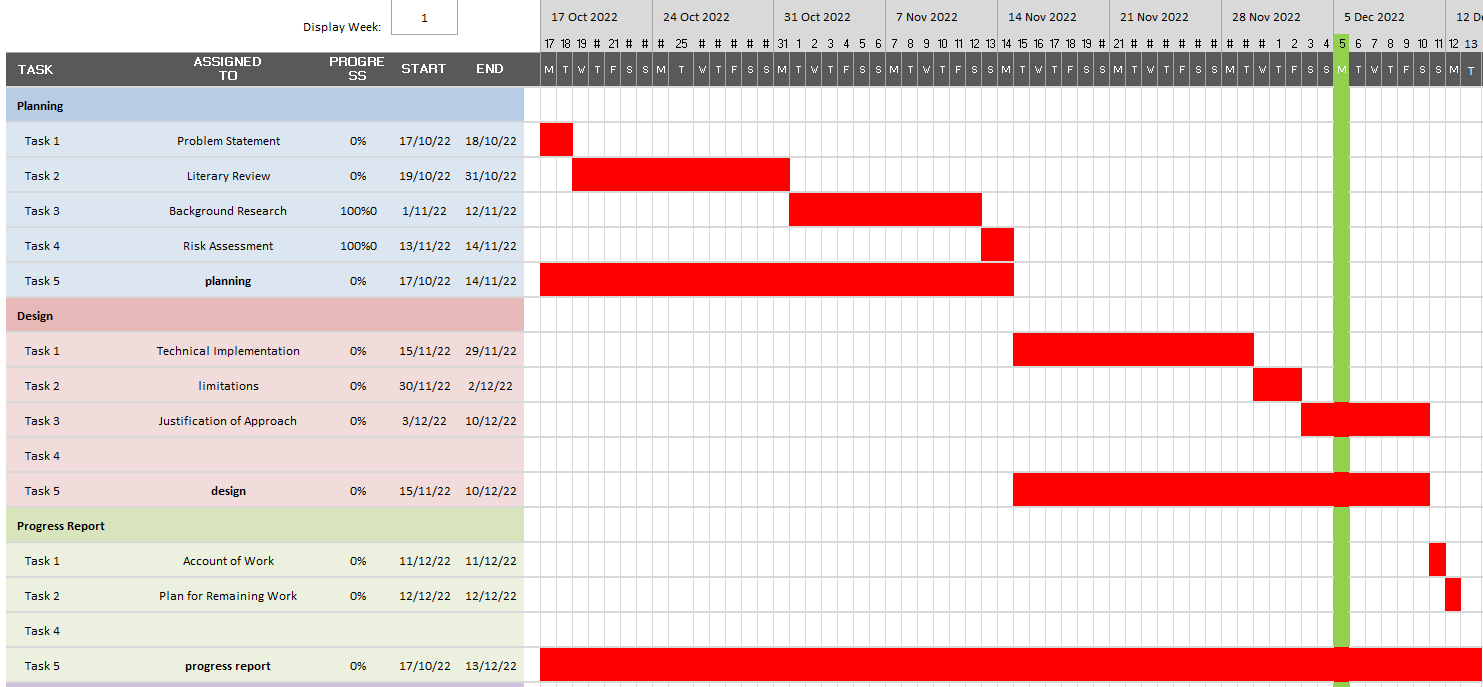
\includegraphics[width=\textwidth]{images/charts/gantt-chart-1.png}\vspace{-4mm}
  \caption{\textit{A Gantt chart for my work up until the progress report.}}
\end{figure}

\section{Plan of Future Work}

\paragraph{Implementation \& Testing}
This phase I will use the agile development methodology to build my application. My sprints will all be structured into three phases:

\begin{enumerate}
  \item \textbf{Preparation} Deciding on the set of requirements to complete and making any initial design decisions and diagrams,
  \item \textbf{Implementation} using test-driven development, I will work on requirements based on their prioritization, and
  \item \textbf{Review} I will discuss the completed work in that sprint including design choices, what was completed, and any issues.  
\end{enumerate}

\paragraph{Testing Strategy and Results}
This phase will be used to discuss my strategy for testing and how it affected the overall success of my project. This will also be supplemented by a series of test results that show how my application fared against the tests I ran, including a discussion on any noteworthy test results. 

\paragraph{Evaluation}
This phase will focus on me critically reflecting aspects of my project and will be used to discuss questions such as:

\begin{itemize}
  \item How does my application fare as a solution to the initial problem?
  \item What changes to the application would make it more successful?
  \item What are the limitations of the application?
  \item What issues did I have during this project?
  \item If I were to do this project again, what would I change?
\end{itemize}
